\documentclass[11pt]{article}
\usepackage[margin=0.8in]{geometry}

\usepackage[comma]{natbib}
\usepackage{color}
\usepackage{mdwlist}
\usepackage{graphicx}
\usepackage{url}
\usepackage{epigraph}
\usepackage{comment}

\setlength{\parskip}{1ex plus 0.5ex minus 0.5ex}
% set width for \epigraph{}{}
\setlength{\epigraphwidth}{.8\textwidth}

\newcommand{\TODO}[1]{\begin{quotation}\noindent\color{blue}\textbf{ToDo}: #1\end{quotation}}

%  Abbreviations for cross-references
\newcommand*{\figref}[1]{Figure~\ref{#1}}
\newcommand*{\tabref}[1]{Table~\ref{#1}}
\newcommand*{\secref}[1]{Section~\ref{#1}}
\newcommand*{\eqref}[1]{Eqn.~(\ref{#1})}

% abbreviations
\newcommand{\Cent}[1]{#1$^{th}$ century}
%\newcommand{\keywords}[1]{\par\noindent\textbf{Key words:} #1}
\newcommand*{\boldital}[1]{\textit{\textbf{#1}}}
%\newcommand*{\epigraph}[2]{{\renewcommand{\baselinestretch}{1}\normalfont\emph{#1}\hfill---#2\par\vspace{1ex}}}
\newcommand*{\degree}[1]{\ensuremath{{#1}^{\circ}}}

\newcommand*{\scat}{scatterplot}
\newcommand*{\scats}{scatterplots}
\newcommand*{\scatmat}{scatterplot matrix}
\newcommand*{\scatmats}{scatterplot matrices}

%\bibliographystyle{abbrvnat-last}
\bibliographystyle{abbrvnat-apa-nourl}
\providecommand{\Loc}[1]{\textsf{#1}}

\begin{document}

\title{The Milestones Project: \\ A Database for the History of Data Visualization}
\author{Michael Friendly \and Matthew Sigal \and Derek Harnanansingh}
\date{\today}

\maketitle

\begin{abstract}
Approaches to modern data visualization have evolved substantially from the first thematic maps of the 1600s and the
first bar charts and line graphs
in the early 1800s to the dynamic and interactive graphics of today.
Over the course of this history, scholars have taken a variety of approaches to show how particular factors of interest have changed over time.

The purpose of this chapter is threefold: first, to introduce the reader to an online resource called the Milestones Project. This website highlights important events in the history of data visualization, and enables users to interactively travel through time to see and explore
the context that surrounded their developments. Secondly, we present some visual
examples that
deal with conveying aspects of history
over time, drawn from this resource and discussed in terms of their goals, similarities, and differences.
Finally, the Milestones database itself will be used to showcase how such a resource can serve as an interesting source of information for statistical historiography, which entails the use of statistical and graphical methods for the analysis and understanding of historical innovations, developments, and trends.
\end{abstract}


\section{Introduction}\label{sec:intro}
\epigraph{If you would understand anything, observe its beginning and its development.}{Aristotle}

Questions regarding the history of data visualization are (or at least should be) of great importance to historians of science, to current developers of graphical methods for statistical analysis and the related info-vis community, as well those just interested in the history of ideas. In the history of science, diagrams, graphs, maps and other visualizations have often played important roles in discoveries that arguably might not have been achieved otherwise.%
\footnote{
	Some salient examples are:
	Francis Galton's 1861 discovery of anti-cyclonic movement of wind around low-pressure areas from contour maps; Edward Maunder's ``butterfly diagram'' of the variation of sunspots over time leading to the	discovery of the ``Maunder minimum,'' from 1645--1715; and Henry Moselely's 1913 discovery of the concept of atomic number, based largely on graphical analysis (a plot of serial numbers of the elements vs. square root of frequencies from their X-ray spectra).
}
At the same time, in the fields of statistical graphics and information visualization, developers often create ``new'' methods without any appreciation that they have deep roots in the past.%
\footnote{
  For example, mosaic displays for frequency tables were thought to have been invented by \citet{HartiganKleiner:81} and extended to show the pattern of residuals in loglinear models by \citet{Friendly:94a}. But it turns out that the essential idea behind this area-based display is goes back to Georg von Mayr in 1877 \citep{Friendly:2002:mosahist}.
}

These two perspectives provided the motivation for the development of the Milestones Project. 
\begin{comment}
Rephrase the second sentence: Previous historical accounts of events, ideas and techniques that relate \emph{inter alia} to modern data visualizations were fragmented - scattered across a wide number of fields, publications, and languages (insert footnote here).  The present project's goal was to bring these resources together into a publicly and freely available database.
\end{comment}
This stemmed from the fact that historical accounts of events, ideas and techniques that relate \emph{inter alia} to modern data visualization were fragmented and scattered across a wide number of fields.%
\footnote{
Among these are general histories in the fields of probability \citep{Hald:1990}, statistics \citep{Pearson:1978,Porter:1986,Stigler:1986}, astronomy \citep{Riddell:1980}, cartography \citep{WallisRobinson:87}. More specialized accounts focus on the early history of graphic recording \citep{HoffGeddes:1959,HoffGeddes:1962}, statistical graphs \citep{Funkhouser:1936,Funkhouser:1937,Royston:1970,Tilling:1975}, fitting equations to empirical data \citep{Farebrother:1999}, cartography \citep{Friis:1974,Kruskal:1977}, thematic mapping \citep{FriendlyPalsky:2007,Palsky:1996,Robinson:1982}, and so forth.
}

When this work began in the mid-1990s, there were no accounts or resources that spanned the entire development of visual thinking and the visual representation of data across different disciplines and perspectives. The Milestones Project began simply as an attempt to collate these diverse contributions into a single, comprehensive listing, organized chronologically, that contained representative images, references to original sources, and links to further discussion -- a source for ``One-Stop Shopping'' on the history of data visualization.

In \secref{sec:project}, we describe the evolution and structure of the Milestones Project. \secref{sec:vistime} presents some historical and modern approaches to one self-referential question: how can data visualization be applied to its own history? \secref{sec:historiography} introduces another self-referential topic we call \emph{statistical historiography}, which entails the use of statistical and graphical methods for the analysis and understanding of historical innovations, developments, and trends. But first we give some brief vignettes of historical topics and questions for which the Milestones Project has proved invaluable in our own research.

\begin{comment}
\begin{itemize*}
 \item The first statistical graph?
 \item Who invented the scatterplot?
 \item The origin of mosaic displays
 \item The Golden Age of statistical graphics
\end{itemize*}
\end{comment}

\subsection{The first statistical graph}
In the history of statistical graphics \citep{Friendly:06:hbook}, as in other artful sciences, there are a number of inventions and developments that can be considered ``firsts'' in these fields. The catalog of the Milestones Project \citep{FriendlyDenis:01} lists 70 events that can be considered to be the initial use or statement of an idea, method or technique that is now commonplace, but there is probably no question more fundamental than that of the first visual representation of statistical data.

In \citet{Friendly-etal:2010:langren} we argue that the 1-dimensional line graph shown in \figref{fig:langren-google-overlay} by Michael Florent van Langen \citep{Langren:1644} should be accorded this honour. The graph shows 12 estimates of the distance in longitude between Toledo and Rome, overlaid on a modern map. van Langren used this to demonstrate that these estimates were all subject to large errors and to
propose to King Phillip of Spain that only he had a sufficiently precise method for the determination of longitude for navigation at sea.

\begin{comment}
I've updated this image to make it clearer.  I didn't like how the original text got lost among the Google Maps text before.
\end{comment}

\begin{figure}[htb]
 \centering
 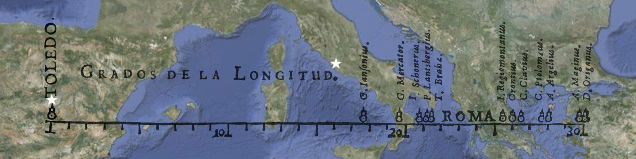
\includegraphics[width=\textwidth]{fig/langren-google-overlay2}
 \caption{van Langren's 1644 graph, re-scaled and overlaid on a modern map of Europe. Toledo is located at lat/long %39$^o$51$^'$36$^\"$N, 4$^o$01$^'$48$^\"$W
(\degree{+39.86}N, \degree{-4.03}W), Rome is located at (\degree{+41.89}N, \degree{+12.5}W), both shown by markers on the map.  This image makes clear what van Langren wished to communicate: the wide variability of the estimates, but also shows how far the estimates were biased.}%
\label{fig:langren-google-overlay}
\end{figure}

The telling of van Langren's story not only turned out to involve astronomy, archival research, details of patronage in the \Cent{17}, and even an unsolved problem of cryptography, but also serves as an example of statistical historiography.  The Milestones Project provided the infrastructure for this research -- through the use of a time-based, cross-referenced catalog of images, references and links to related work, van Langren's tale was able to be studied and reported upon.

\subsection{Who invented the scatterplot?}
Although there are earlier precursors, the main graphical methods used today --
pie charts, line graphs and bar charts -- are generally attributed to William Playfair around the beginning of the \Cent{19} \citep{Playfair:1786,Playfair:1801}. Each of these are essentially univariate displays, showcasing some aspect of a single variable. 

A logical next step would be to discover a method that could reveal the relationship between two variables, which we now know as the scatterplot.  By \citeyear{Galton:1886}, Francis Galton had utilized this truly bivariate display in his discovery of correlation and regression, and it would become an essential tool for the presentation of multivariate statistics. However, he may not have been the first to use this graphical technique, and it is surprising that no one is widely credited with its invention.

In \citet{FriendlyDenis:05:scat}, we delved into this mystery.  This involved tracing the early origins of ideas related to the scatterplot, which led to two compelling narratives: how, in Playfair's time, it was nearly impossible to think about and visualize bivariate relationships; and, later, how the scatterplot was quintessential for Galton's visual insights that would lead to the rise of modern statistics and graphics. It was the resources available in the Milestones Project that allowed us to focus upon the events between these two extremities and attribute the essential ideas of the scatterplot to J. F. W. Herschel in two 1832 papers.

\subsection{The Golden Age of statistical graphics}

In our initial web presentation of the Milestones Project, it proved convenient
to sub-divide the history of data visualization into epochs, each of which turned
out to be describable by coherent themes.  For reasons we describe later, one
period turned out to be particularly noteworthy, both for the sheer number of
contributions, and for the beauty and elegance of their execution. We call this period, from roughly 1850 to 1900 ($\pm 10$), the Golden Age of statistical graphics \citep{Friendly:2008:golden}.

\figref{fig:mileyears4} shows the time distribution of the 260 significant events that had been included in the Milestones Project database by 2007, demarcated by the labels we used for epochs. In \citet{Friendly:2008:golden}, we traced the origin of this period in terms of the infrastructure required to produce such an explosive growth of contributions to data visualization, and found three primary sources: the systematic data collection by state agencies, the rise in popularity of statistical and visual thinking, and the enabling developments of technological innovations.
%% one figure
\begin{figure}[!htb]
  \centering
  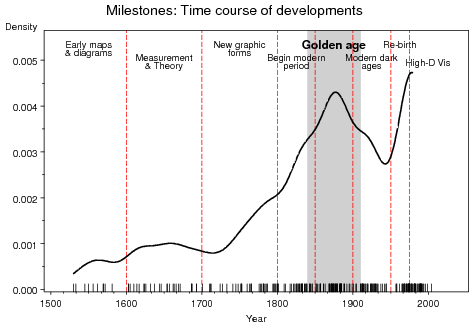
\includegraphics[width=.9\textwidth,clip]{fig/mileyears4}
  \caption{The time distribution of events considered milestones in the history of data visualization, shown by a rug plot and density estimate. The density estimate is based on $n=260$ significant events in the history of data of data visualization from 1500--present. The developments in the highlighted period, from roughly 1840--1910 comprise the Golden Age of statistical graphics.}
  \label{fig:mileyears4}
\end{figure}
\section{The Milestones Project}\label{sec:project}
An early overview of the content and aims of the Milestones Project appeared in \cite{Friendly:04:gfkl}.
Here we update that description and provide a few technical details on some problems in
documenting the history of data visualization in a convenient form for browsing, searching and
analysis.

\subsection{Origin, structure and evolution}\label{sec:structure}
The initial step in portraying the history of data visualization was a simple chronological listing of milestone items
with capsule descriptions, bibliographic references, markers for date, person, place, and links to portraits, images,
related sources or more detailed commentaries.
We started with 105
developments listed by \citet{BenigerRobyn:1978}
and incorporated additional listings from
\citet{Hankins:1999},  \citet{Tufte:1983,Tufte:1990,Tufte:1997},  \citet{Heiser:2000}, and others.

This began as single \LaTeX\ file (with markup tags for all relevant bits of information),
used to produce a
hyper-linked PDF document.  A variety of software tools (perl scripts, Unix utilities) allowed us to turn this
single source
\emph{directly} into the web version originally shown at
\url{http://www.math.yorku.ca/SCS/Gallery/milestone}.  Other custom software tools allowed us to
add new milestones items from text files using a template of tags (DATE:, AUTHOR:, WHAT:, REF:, IMG:, etc.)
and extract the
information about milestones items, authors, images, etc. in a variety of forms (CSV, XML, JSON)
that could be used as input for analyses and graphic displays.  For example, \figref{fig:mileyears4}
was produced in SAS software using a unix command pipe like
\begin{verbatim}
itemdb -o milestones.csv < milestones.tex | sas -i milestones.csv mileyears.sas
\end{verbatim}

\begin{figure}[!htb]
  \centering
  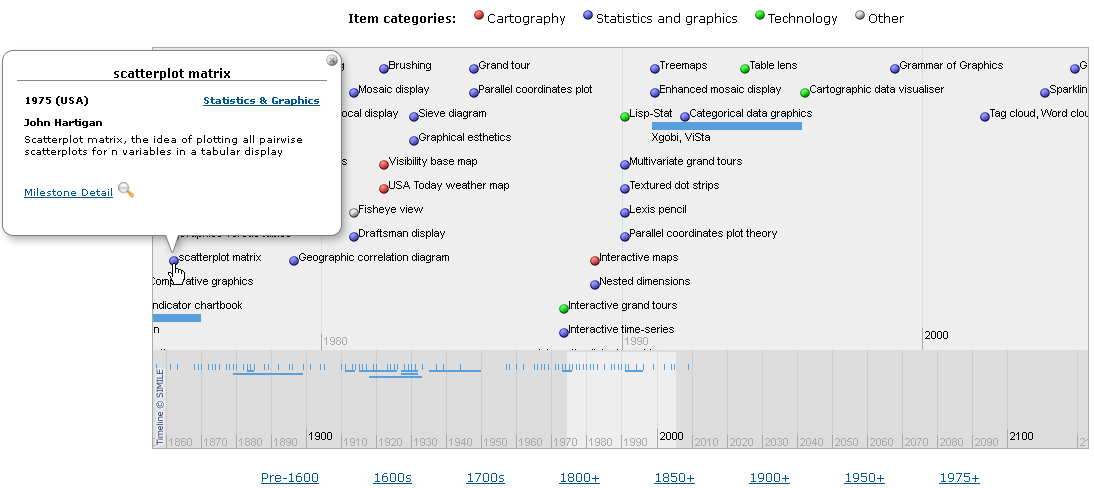
\includegraphics[width=\textwidth,clip]{fig/datavis-timeline2}
  \caption{Timeline view of the Milestones Project on the site \texttt{http://datavis.ca}. In this view,
  the top panel shows a detailed view of the segment of history highlighted in the bottom panel, both
  of which can be separately scrolled. Items in the top panel show a brief tag, color-coded in coarse
  categories. Clicking on an item in this panel brings up small description, linked to the details of
  the milestone item.
  }
  \label{fig:datavis-timeline2}
\end{figure}

It soon became apparent that such a text-based representation was inadequate. Updating the milestones data 
required that the single \LaTeX\ file be shared between multiple collaborators over email, and milestones 
assets, such as images or URLs were stored on a single computer not easily accessible by other collaborators.
As a result, collaboration with more than a few collaborators was cumbersome. The single file needed to be vetted 
at each iteration, and once enough data had been collected, rendered into a web site and manually uploaded so
that non-collaborators, namely the public, would be able to view the data.

Around 2005, we began to convert the flat file into a relational data and completely redesign the Milestones 
web site. Specifically, we wanted to facilitate collaboration between any number of collaborators via an easy
to use web administration area and allow for the dissemination of milestones data via an easy to browse public 
user interface, both of which would be tied to a relational database.

Migrating the data to this form provided some challenges. First, the existing milestones data needed to be
normalized and redundancy minimized. To do this, we broke the data into its relavent entities namely the 
milestone itself and its descriptors (aspect, author, subject, keywords, reference, and mediaitem).
The aspect, author, subject, keyword and reference descriptors exist as a many-to-many relationship between 
it and the milestone. For example an aspect can belong to one or more milestones and the mileston can belong to 
one or more aspects. While media items on the other hand, can belong to only one milestone at a time, with
multiple mediaitems possible for a single milestone. \figref{fig:datavis-schems-2} describes these relationships.

Normalizing the data in this way enabled us to free the databse of modification anomalies; ensured that database 
structure was scalable and could be extended with minimum mofications; made the relational model more informative 
to users; and made sure the data itself was query-neutral (Codd, 1971).

The second challenge related to how to display such a vast amount of information in an easy to understand
user interface...



\begin{figure}[!htb]
  \centering
  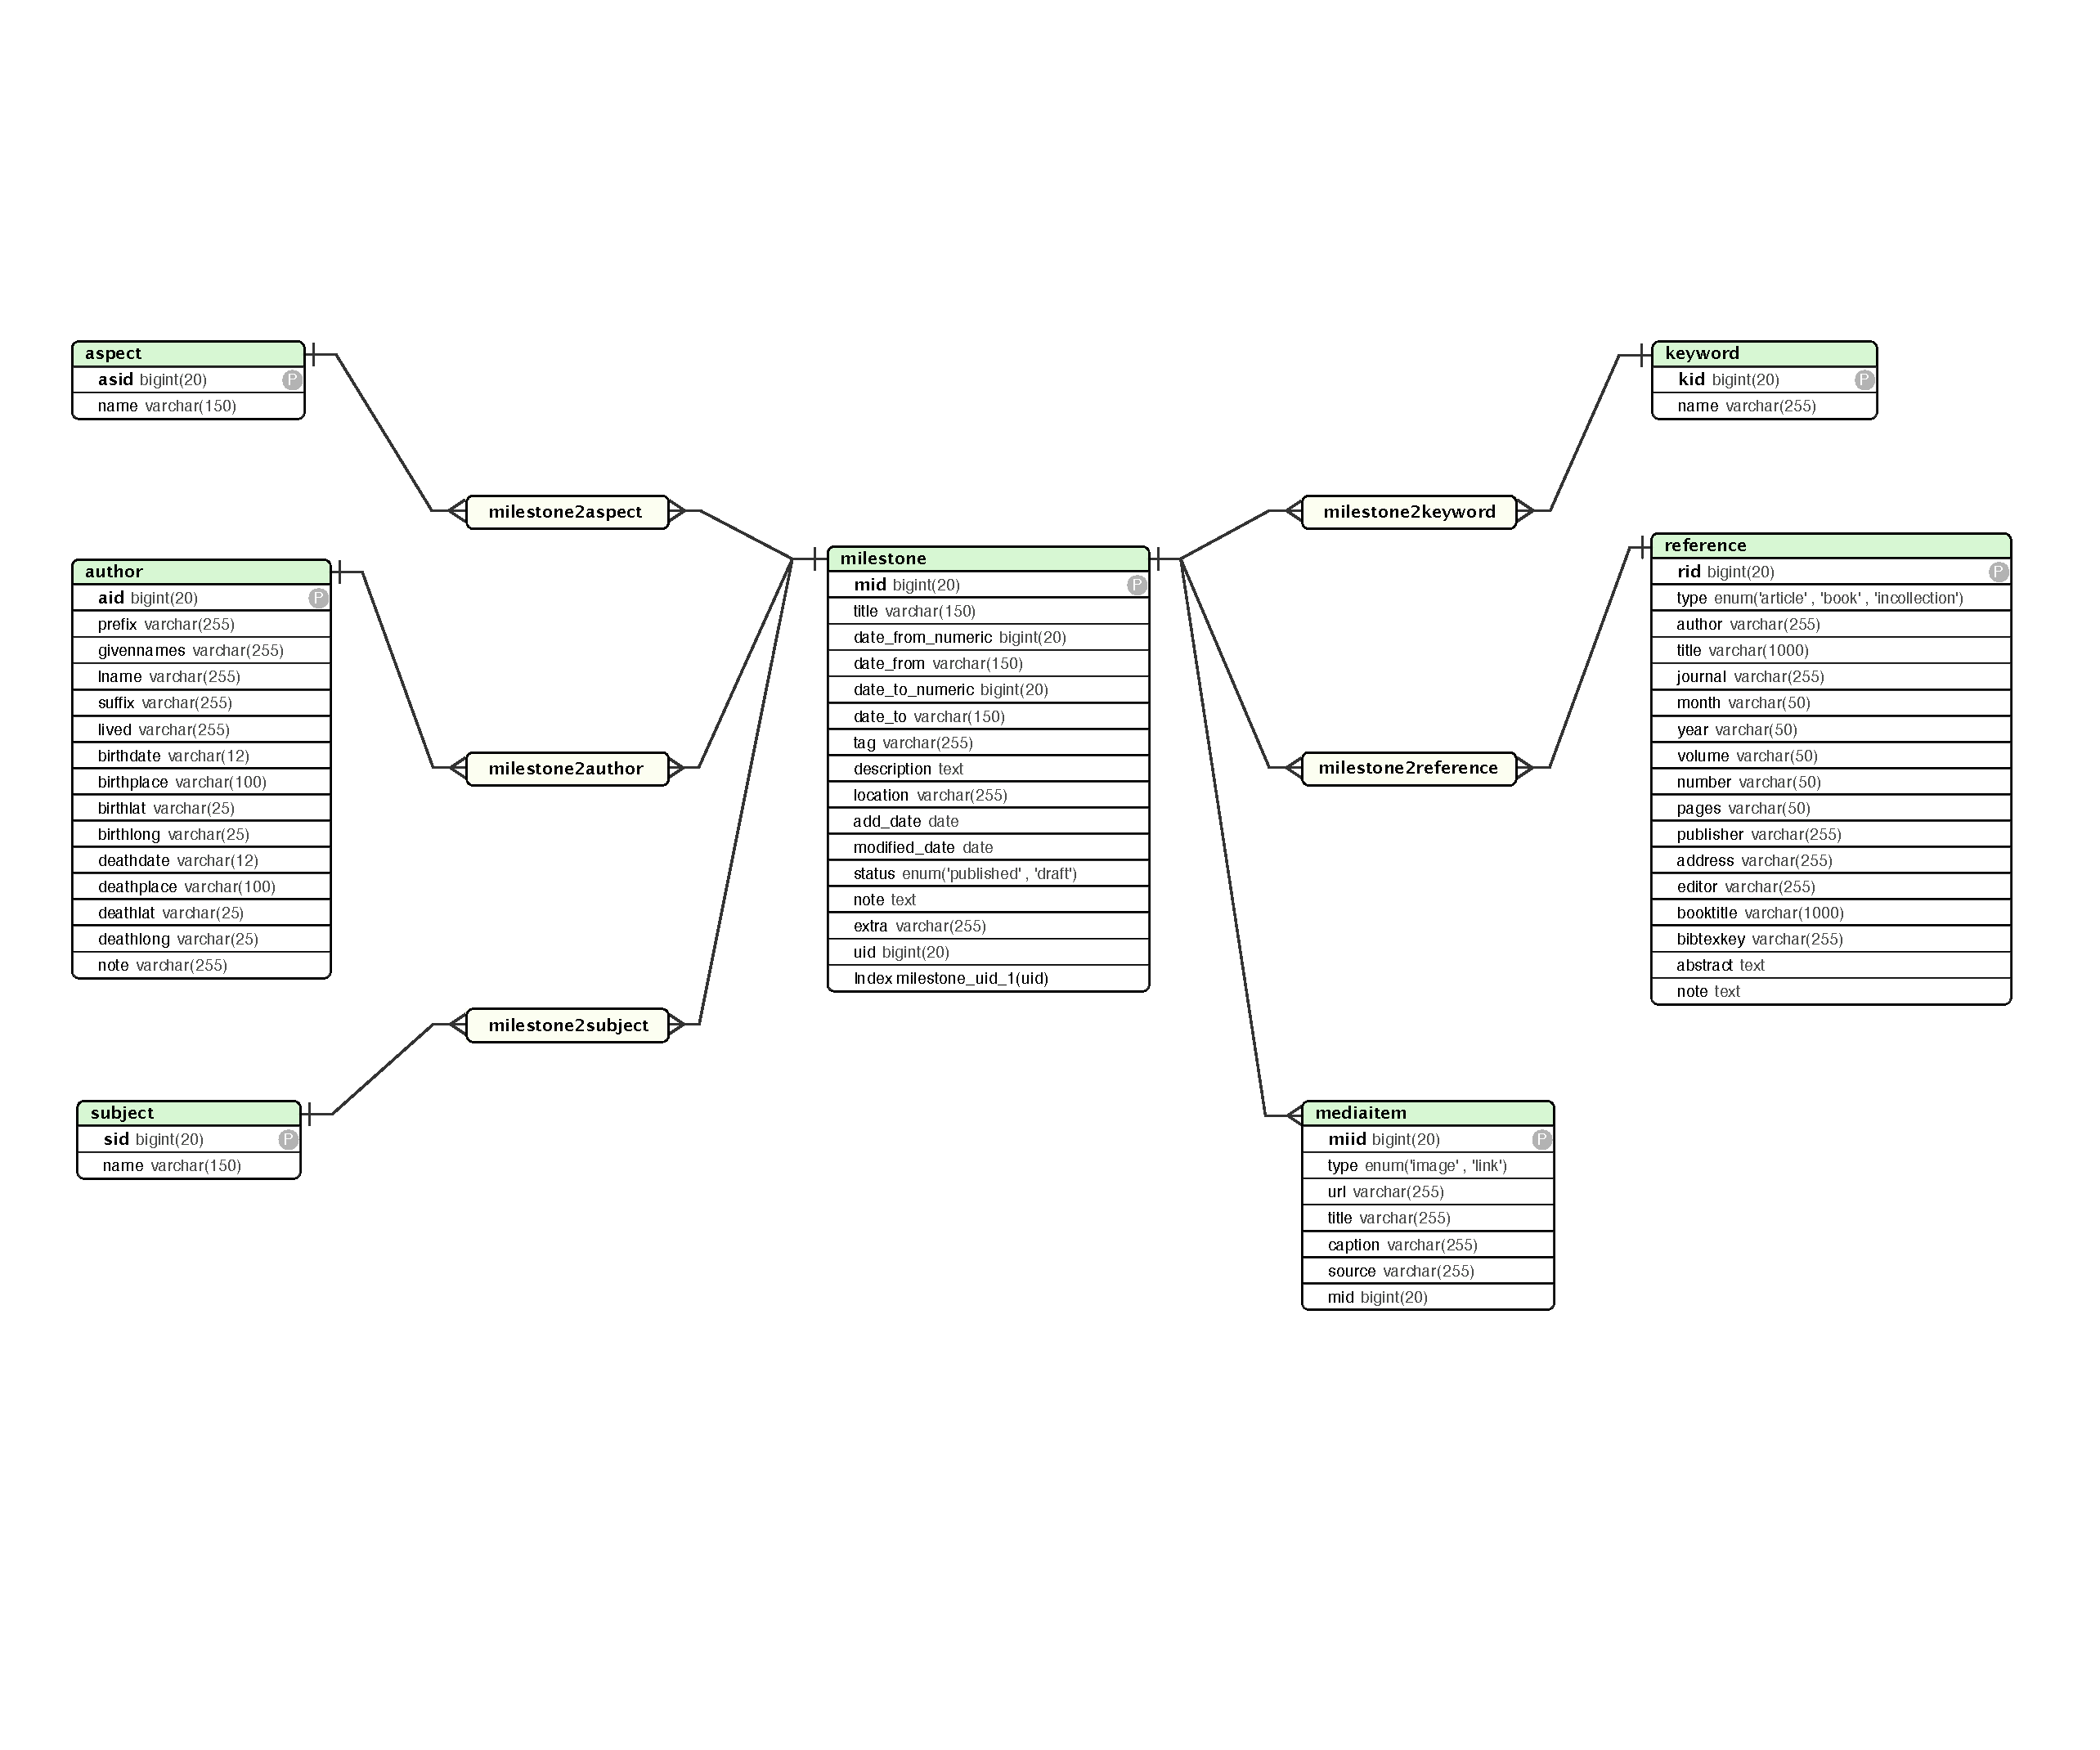
\includegraphics[width=\textwidth,clip]{fig/datavis-schema-2}
  \caption{Simplified schema for the MySQL database for the Milestones Project. The main 
  table (\texttt{milestone}) contains information regarding each of the items considered
  a milestone in the history of data visualization, linked to other tables 
  (e.g., \texttt{reference}, \texttt{mediaitem}) by unique (primary) keys.
  Other supporting tables (e.g., \texttt{milestone2aspect}) provide for convenient lookups of 
  descriptors of these milestones items (\texttt{subject}, \texttt{aspect}, \texttt{keyword}).
  }
  \label{fig:datavis-schema-2}
\end{figure}


At present, the Milestones Project lists 288 contributions to this history, with nearly 350 references,
information on 336 authors and 774 ``media items'', comprising 371 images appearing online on the
\url{http://datavis.ca} site and 403 links to images and documents at other sites.
In addition, we maintain an offline image database comprising over 1100 images collected from
various sources, ...

\figref{fig:datavis-timeline2} shows the timeline view of the miletsones items displayed on the
landing page. 



\section{Visualizing Time: Historical Precedents}\label{sec:vistime}
\begin{itemize*}
  \item Visions of history from the past
  \item Correlated pasts
  \item Non-linear scales
  \item Dynamic/interactive timelines
\end{itemize*}

\epigraph{What does history look like?  How do you draw time?}{\citet[p. 10]{RosenbergGrafton:2010}}
The questions in this quotation from \emph{Cartographies of Time: A History of the Timeline} \citet{RosenbergGrafton:2010}
introduce an important topic in the history of data visualization: how to visualize this history?
Time provides one obvious dimension, but what else can be included to show the details of a history in a static display
or allow users to see more using dynamic and interactive displays?

We have also provided an annotated visual gallery of some timeline designs and visual histories
in our Data Visualization Gallery at \url{datavis.ca/gallery/timelines.php}. ...


\begin{figure}[!htb]
  \centering
  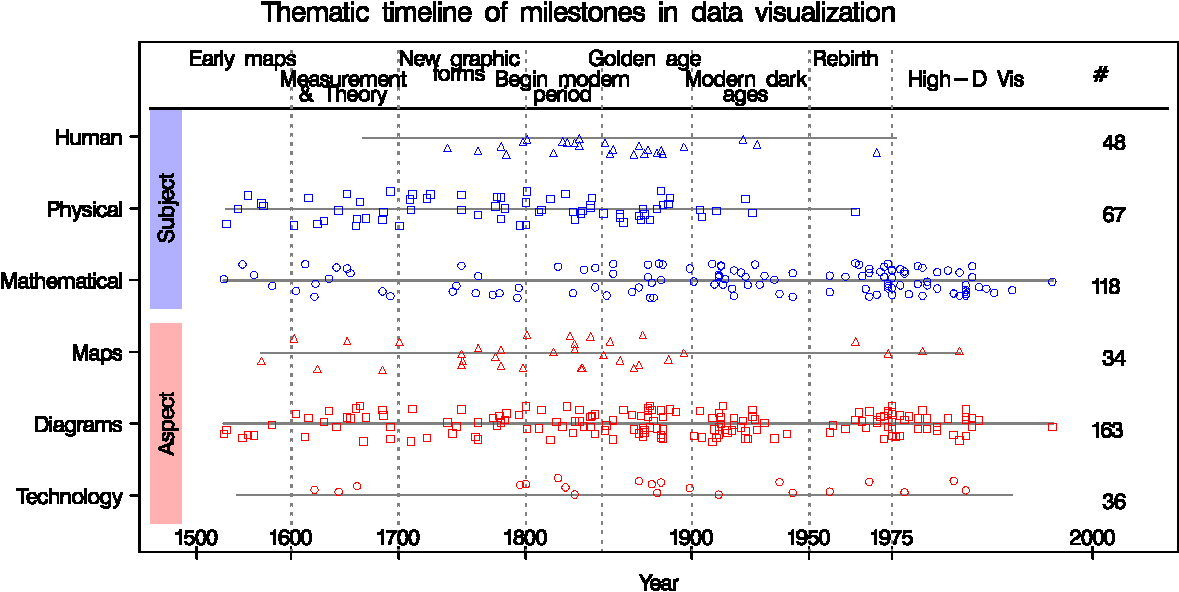
\includegraphics[width=\textwidth,clip]{fig/milecatline}
  \caption{Sketch for a thematic timeline of milestones items, categorized by the Subject (content) 
  and Aspect (form) of the milestone item.  To provide greater resolution for more recent events,
  time (Year) is shown on a square-root scale, going backward from the year 2000.
  }
  \label{fig:milecatline}
\end{figure}




\section{Using the Milestones Project for Statistical Historiography}\label{sec:historiography}
\begin{itemize*}
  \item comparisons of graphical innovations by field (e.g. physical sciences vs. social sciences), in terms of content and form
  \item extract themes and relationships between content areas
\end{itemize*}

\subsection{Statistical historiography}\label{sec:stathist}
We use the term ``statistical historiography,''
to refer to the use of statistical and graphical methods to
explore, study and describe historical problems and questions.%
\footnote{As far as we know, the initial expression of this idea appeared in a paper by
\citet{Rubin:1943} discussing various ways in which statistical methods could be applied
to historical topics.  These included the use of sampling methods to test historical theories,
statistical distributions applied to historical data, and the use of
time series graphs with smoothed curves to study historical trends.
More recently, many examples of the application of these ideas to statistical topics
can be found in \citet{Stigler:1986,Stigler:1999}, as well as our own papers
on the history of data visualization,
cited \emph{inter alia}.
}
This topic has a delightful self-referential quality when applied to the history of data visualization itself,
since we have often found ourselves using modern methods of statistical analysis and graphics to study
the development of ideas in this area.

At the same time, our examination of some of the most
impressive graphic works of the past sometimes left us awe-struck by their exquisite
beauty and visual design.%
\footnote{ Some examples are:
Charles Joseph Minard's famous depiction of Napoleon's March on Moscow \citep{Friendly:02:Minard},
Francis Galton's detailed study of weather patterns in Europe \citep[see:][]{Friendly:2008:golden},
and Andr{\'e}-Michel Guerry's \citep[Plate 17]{Guerry:1864}
semi-graphic table depicting the relations of occurrence of
crimes to a wide variety of social and demographic factors \citep[see:][]{Friendly:2007:guerry}
...
}
On more than one occasion, we wondered whether there wasn't something lost with the advent of modern
software: We can now analyze massive data sets and generate many graphs with simple mouse clicks
or software commands, but designing a truly effective graphic display requires much thought and
a lot of manual intervention.

There is, of course,  one principal requirement for statistical historiography: \textbf{data}.
The milestones database is the repository of all the information we have so far recorded,
and modern database tools allow the possibility of simple or complex queries, limited only
by the available information.

In related work, we have also collected and disseminated
data sets of historical interest on a variety of
topics in statistics and data visualization, for example in the R packages
HistData \citep{HistData} and Guerry \citep{Guerry}.

In the subsections below, we describe a few applications of these ideas using the milestones
database and case studies that arose from this work. There is an interesting interplay between
such historical analyses and these data collections. Some studies called for us to find and
incorporate new data sources, such as our paper \citep{Friendly:2007:guerry} on
Guerry's \emph{Moral statistics of France} and the Guerry package to which we added
Angeville's 1836
extensive data on social and economic characteristics of France.
In other cases, our analyses suggested new or different ways to visualize historical data.

\subsection{Milestone authors: lifespan}\label{sec:lifespan}
As noted earlier, we record information relevant to the contributors of milestones events in an
author table in the database. Internet and biographical searches for these persons allowed us
to determine the dates and places of their birth and death in a large number of cases.

\begin{figure}[!htb]
  \centering
  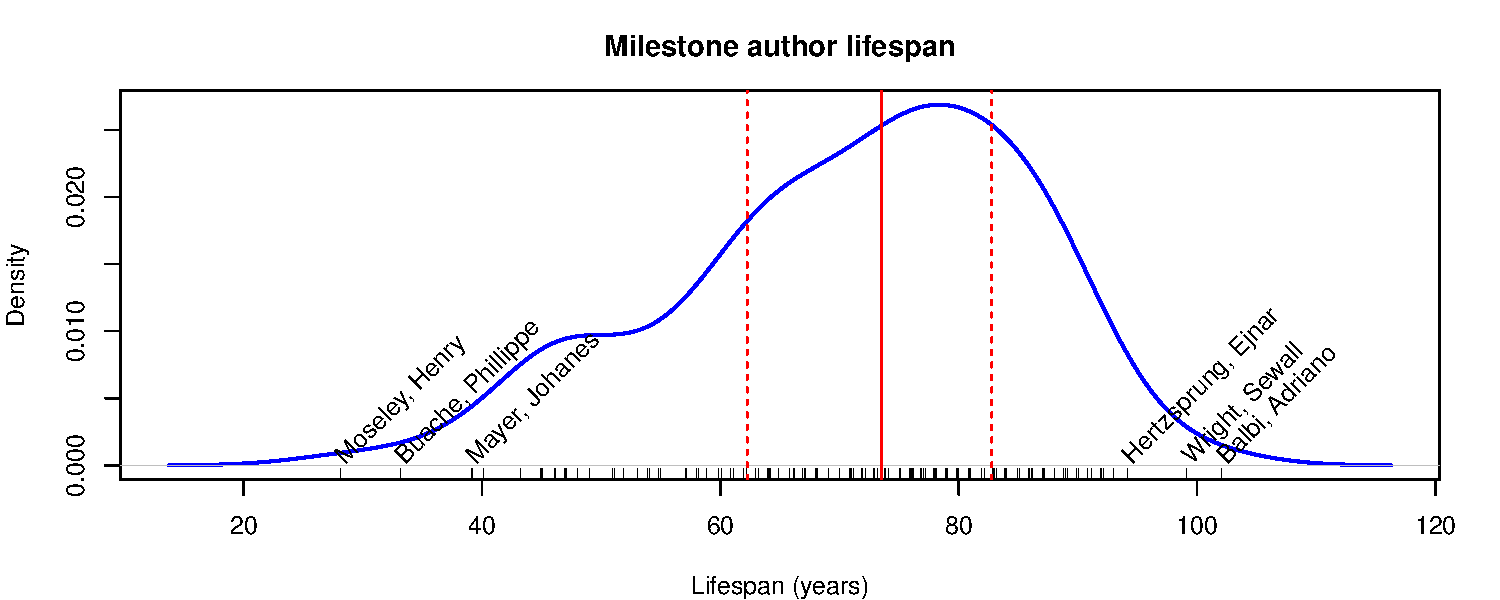
\includegraphics[width=\textwidth,clip]{fig/lifespan}
  \caption{Density plot of the lifespan of 172 authors in the milestones database born after 1500 and for whom
  lifespan can be determined. Individual observations are shown by a (jittered) rug plot, and the three extremes
  on each end are identified by name.  The dashed lines show the quartiles of the distribution.
  }
  \label{fig:lifespan}
\end{figure}

One simple question is how long did these contributors live? As illustrated earlier (figref:)
Joseph Priestley was the first to develop the idea of using a graphic representation to show
the lifespan of famous men. His ``charts of biography'' did this in a particularly evocative
form, showing each person by a line segment identified by name, and grouped into
occupational categories.

However, such ``lifeline'' charts don't provide any answers to this question.  With the
author table, it is a simple matter to calculate lifespan, and give a direct answer
with the help of software.  \figref{fig:lifespan} shows one display of this information,
using a combined density plot and rug plot, as we used in \figref{fig:mileyears4}.

Several features of this plot deserve comment, and also invite further inquiry:
Most notable is that, by and large, milestones authors generally lived to a ripe old age--
the median lifespan is 73.0, but the density plot peaks at around 79.
This contrasts with a detailed study by
David de la Croix and Omar Licandro (\url{http://www.fcs.edu.uy/archivos/BCU_clebrities.pdf})
of famous people from 2400 BC to 1880 AD,
fluctuating around a mean of 61 years for 4 millennia, and only reaching a mean of 69 years
by the end of their sample. To take this analysis further would require more data, for example
a classification of authors by occupational groups.

Second, there is a noticeable bump in the distribution around 45 years. This
occurrence also calls for some attempt at further explanation.
We don't pursue this here, but again note that such graphs often suggest
further analyses (breakdowns by region or time period)
or cry out for the collection of more data.

Finally, although \figref{fig:lifespan} is just a summary graph, we have labeled a few
extreme observations on each end, which may relate to telling parts of the story of the
history of data visualization.  Among these, Henry Moselely, who is known for the
discovery of atomic number from a graphical display, died the youngest, as a consequence
of serving in the British Army in World War I. But, we were surprised to see
the noted and prolific French cartographer Phillippe Buache
and the German physicist and astronomer Johann Tobias Mayer show up in positions
2-3.  On the other end, we were delighted to see that Adriano Balbi,
a Venetian geographer and early collaborator of Andr{\'e}-Michel Guerry
\citep{BalbiGuerry:1829} had the longest lifespan,
just exceeding the population geneticist, Sewall Wright, who invented
path analysis and the path diagram around 1920.

\subsection{Milestone authors: geography}\label{sec:geography}
The Milestones Project web site provides an initial page showing an interactive timeline
of the events events in this history as a visual overview (\figref{fig:mileyears4}).
A long-term goal has been to
provide other views of this history and other tools for searching and exploring the
database.

The geography of these developments so far is only represented in the birth place
and death place information we recorded in the author table.
For example, we know that Minard was born in Dijon, and died in Bordeaux, but
all of his work was done in Paris while he worked at the
{\'E}cole Nationale des Ponts et Chauss{\'e}es.

Nevertheless, a geographic view of the available information is potentially useful.
In this regard, we used the Google geocoding tools to provide latitude and
longitude for the place names listed in the author table.  Using this and the
R package googleVis \citep{googleVis} we easily created the interactive map shown
in \figref{fig:authormap}

Like other Google maps, this can be panned and zoomed using mouse controls.
The place markers display tool tips when hovered and, when clicked, link to
a search page showing milestone items related to that author.
This tool seems sufficiently useful that we are adding it as another visual
overview page to the milestones site.


\begin{figure}[!htb]
  \centering
  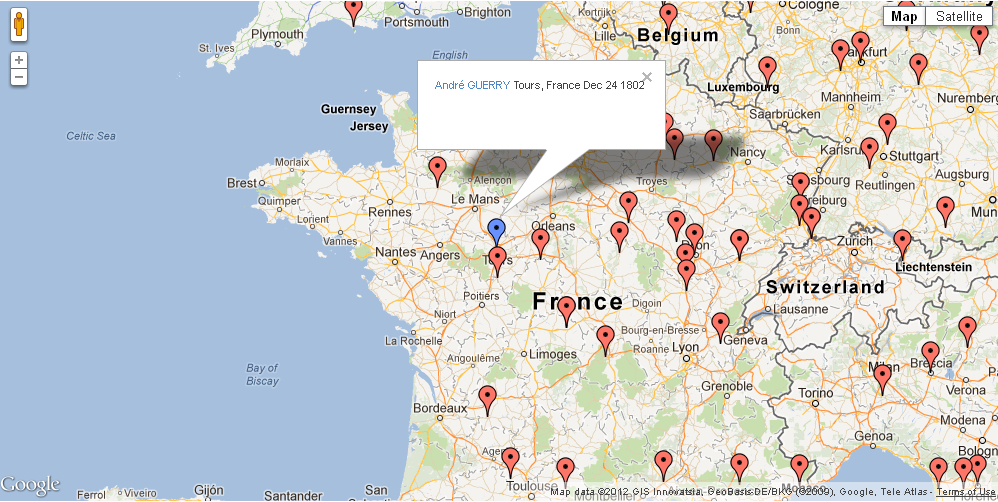
\includegraphics[width=\textwidth,clip]{fig/authormap}
  \caption{Birth places of 188 milestones authors, shown on an interactive Google map, zoomed to show locations
  in part of Europe centered on France. Each geographic marker is linked to a query on
  the \texttt{datavis.ca} web site listing the contributions by that author.
  }
  \label{fig:authormap}
\end{figure}



\section{Conclusion}
-Summarize and conclude

\bibliography{graphics,timeref,Rpackages}
%\bibliography{references}        % after being processed by aux2bib 
%\bibliography{FriendlySigal2012}        % after being processed bibtool -- quiet=on -r ~/texmf/bibtex/bib/aux2bib.rsc -x FriendlySigal2012.aux -o FriendlySigal2012.bib
\end{document} 